\documentclass[8pt]{beamer}
\usepackage{tikz}
\usepackage[utf8]{vietnam}
\usepackage{amsmath}
\usepackage{graphicx}
\usepackage{wrapfig}
\usepackage{hyperref}
\usetheme{Copenhagen}
\usecolortheme{dolphin}
\setbeamertemplate{navigation symbols}{}
\setbeamertemplate{headline}{}
\title[Chương 0: Giới thiệu môn học] %optional
{Chương 0: Giới thiệu môn học}
\subtitle{Xử lý tín hiệu số}
\author[Xử lý tín hiệu số] % (optional)
{Tín Vũ}
\date[VLC 2021] % (optional)
{tinvu1309@gmail.com}
\begin{document}
\frame{\titlepage}
\begin{frame}{Mục lục}
\tableofcontents
\end{frame}
\begin{frame}{Giới thiệu playlist}
\section{Giới thiệu playlist}
	\begin{itemize}
		\item Mình là Tín Vũ, hiện đang là sinh viên học tại Trường Đại học Công nghệ, Đại học Quốc gia Hà Nội. Mình tạo playlist video này để hỗ trợ các bạn học môn \textbf{Xử lý tín hiệu số}.
\item Khác với môn học tiên quyết \alert{Tín hiệu hệ thống} trước đó, bài giảng môn học này \textbf{hoàn toàn bám sát với đề cương và giáo trình nội bộ} của trường mình, nên các bạn trường khác cần phải lưu ý rất kĩ điều này.
\item Không chỉ dừng lại ở lý thuyết, playlist này \textbf{có bổ sung hướng dẫn lập trình cơ bản bằng GNU Octave/Matlab} để vẽ phổ tín hiệu, đáp ứng tần số và thiết kế bộ lọc.
\item Môn học này bao gồm \textbf{6 chương}, các chương đều liên quan rất chặt chẽ với nhau nên hãy học cẩn thận ngay từ \alert{Chương 0} để ôn thi cuối kì đỡ vất vả.
	\end{itemize}
\end{frame}
\begin{frame}{Tài liệu tham khảo}
\section{Tài liệu tham khảo}
\begin{itemize}
		\item Tài liệu tham khảo chính: Giáo trình Xử lý tín hiệu số (Nguyễn Linh Trung, Trần Đức Tân, Huỳnh Hữu Tuệ, ĐHCN, 2012).
		\item Tài liệu tham khảo phụ: Discrete-time Signal Processing (Alan V.Oppenheim, 2nd edition). 
	\end{itemize}
\end{frame}
\begin{frame}{Kiến thức cơ sở tiên quyết}
\section{Kiến thức cơ sở tiên quyết}
\begin{itemize}

	\item[-] Môn học cơ sở tối quan trọng bạn cần phải nắm được trước khi học \textbf{Xử lý tín hiệu số} là \alert{\textbf{Tín hiệu và hệ thống}}. Hãy ôn lại ngay toàn bộ kiến thức của môn \alert{\textbf{Tín hiệu và hệ thống}} nếu bạn nắm chưa vững, đặc biệt là phần \textbf{Tín hiệu và hệ thống rời rạc} và \textbf{Biến đổi Z}.
\item[-] Ngoài ra, khả năng tính toán tốt là điểm cộng rất lớn, vì khác với môn học trước ta chỉ xử lý \textit{các bài toán mô phỏng} được thiết kế với hằng số đẹp; môn học này ta sẽ xử lý \textit{các bài toán thực tiễn} nên các con số sẽ lớn và cực lẻ. Hay nói cách khác, tính toán ra kết quả tuyệt đối chính xác là việc bất khả thi.
\item[-] Chính vì thế nên  các phần mềm tính toán như GNU Octave/Matlab hỗ trợ bạn rất hiệu quả trong quá trình học. Bạn nên cài sẵn phần mềm trước khi học môn này vì ta sẽ dùng chúng tương đối nhiều.
\item[-] Các kiến thức rất cơ bản về lập trình GNU Octave/Matlab được tích hợp từ \alert{Chương 3} trở đi.
\item[-] Do cú pháp lập trình của hai phần mềm này rất giống nhau nên mình chỉ sử dụng GNU Octave để tính toán và chạy mô phỏng mà thôi.
\end{itemize}
\end{frame}
\begin{frame}{Quy trình xử lý tín hiệu số}
\section{Quy trình xử lý tín hiệu số}
\begin{figure}[h]
			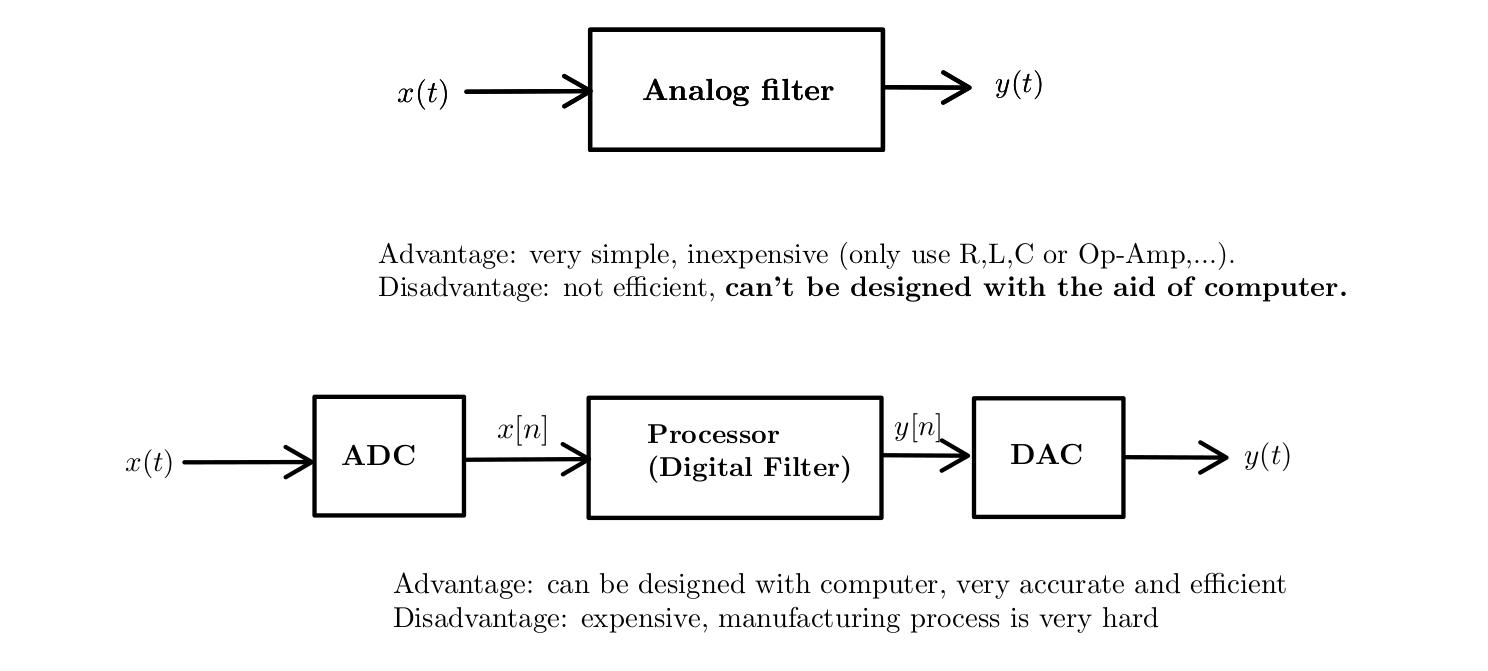
\includegraphics[width=1.1\textwidth]{1.jpg}
			\caption{Discrete-time Signal Processing}			\label{fig:re1}
		\end{figure}

\end{frame}
\begin{frame}{Quy trình xử lý tín hiệu số}
\begin{figure}[h]
			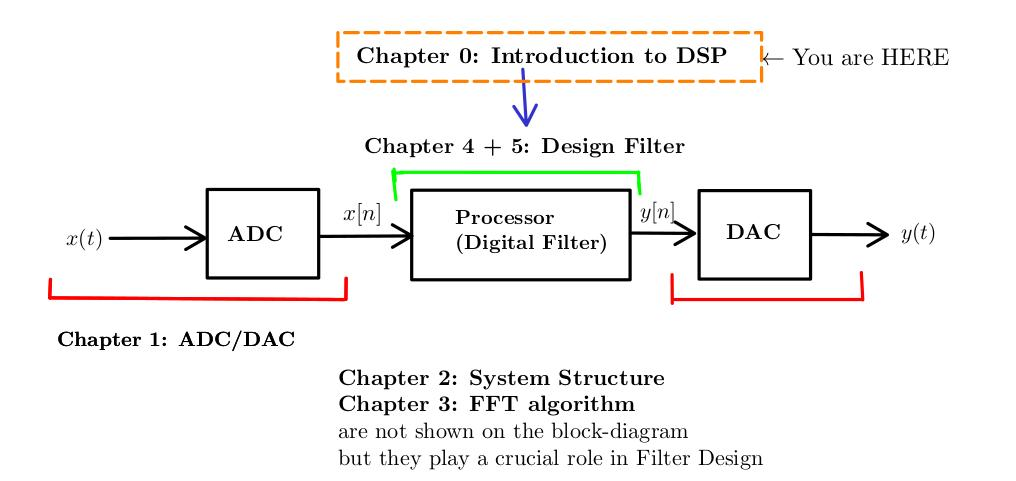
\includegraphics[width=1.1\textwidth]{2.jpg}
			\caption{DSP Learning Process}			\label{fig:re2}
		\end{figure}


\end{frame}
\end{document}
